\section{Class diagram}

This is the class diagram of the current website implementation. As you can see, our current implementation has once again grown significantly thanks to the addition of various classes. \newline

First of all the poule class has replaced the previous group class and is now linked to smaller class such as the Score class which records the score of a match or the pouleStatus class which holds the status of the poule (allowing us to reduce string duplication in database).\newline

Many other small classes have been added to reduce string duplication in database such as CourtSurface, CourtState, courtType and TournoiStatus. Allowing our implementation to become more efficient in it's usage of memory space.\newline

Second, the class UserInWaitOfActivation was added to keep track of user who haven't validated their email after inscription. Allowing us to delete them easily should they not regularise their situation within a given time limit (currently one week). This new class is accompanied with a boolean in participant to allow faster computation, avoiding us to have to check the whole list of user in wait of activation to verify if a participant has been validated or not.\newline

Third, the new log activity class allows us to keep track over every modification as well as the staff member responsible for the modification and the date at which it was made. \newline

Finally the Arbre class which is still a work in progress will shortly allow us to create working knock off tournament as requested in the requirement.\newline

\begin{figure}[!ht]
	\centering
	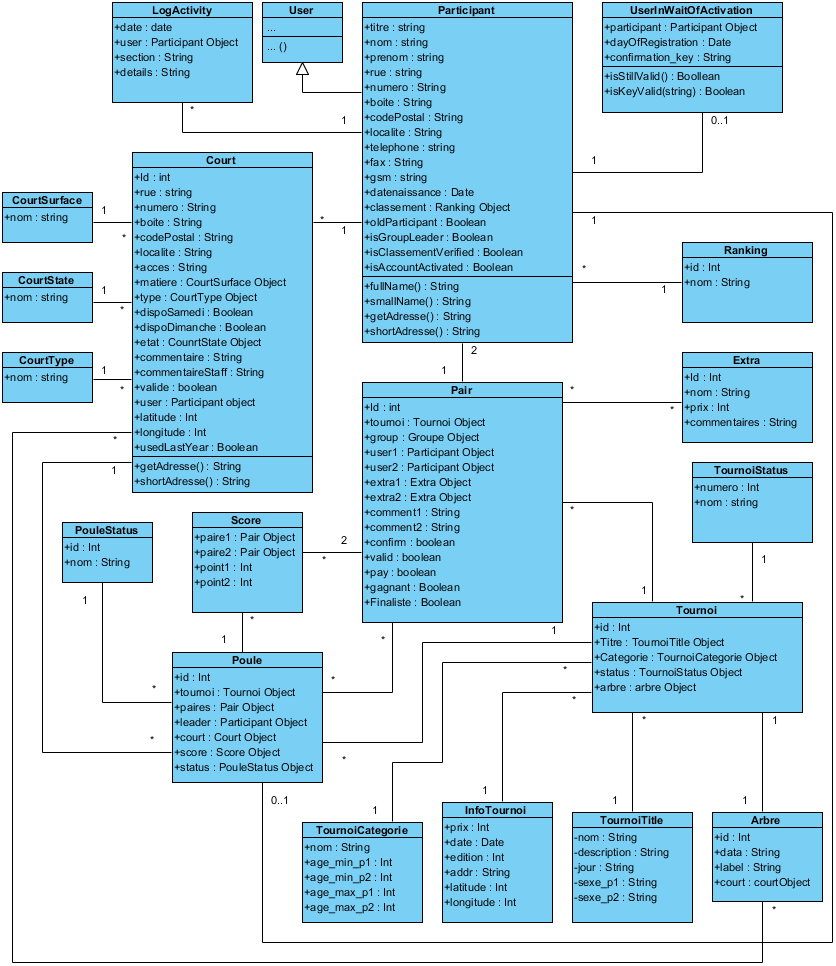
\includegraphics[width=1\linewidth]{class.png}
	\caption{Class diagram of our current implementation}
	\label{fig:length_eight_mouse}
\end{figure}
\FloatBarrier